\فصل{راهکار پیشنهادی}

راهکار پیشنهادی شامل ترکیب بهبود یافته‌ی روش پی.پی.اِم.سی و لولوها می‌شود. این راهکار به طور همزمان دو چالش اساسی در دنیای حریم خصوصی تفاضلی محلی برای داده‌های با ابعاد بالا و در حال تغییر را هدف قرار می‌دهد. در این فصل ابتدا کلیت ساختار الگوریتم و نحوه‌ی عملکرد آن در طول زمان شرح داده‌ می‌شود. سپس جزئیات پیاده‌سازی به تفصیل بیان خواهد شد، در نهایت نیز راهکار پیشنهادی حاضر مورد ارزیابی قرار خواهد گرفت.

\قسمت{بررسی چارچوب راهکار پیشنهادی}

به صورت خلاصه، با استفاده از تبدیل هار تمام داده‌ها به دو جزء میانگین و بردار ویژه تجزیه شده، در فرایند تصادفی‌سازی قرار گرفته و سمت کارپذیر ارسال می‌شوند. مسیر ذکر شده، \مهم{فرایند اصلی} راهکار پیشنهادی را بیان می‌کند. منتها قبل از شروع این فرایند، باید اعمال اضافه‌تری روی داده‌های در حال تغییر انجام داد تا بتوان آنها را وارد فرایند اصلی کرد. شکل \رجوع{fig:thesisClient} به طور کلی رفتار الگوریتم سمت کاربر را نشان می‌دهد.

\begin{figure}[h]
  \centering
  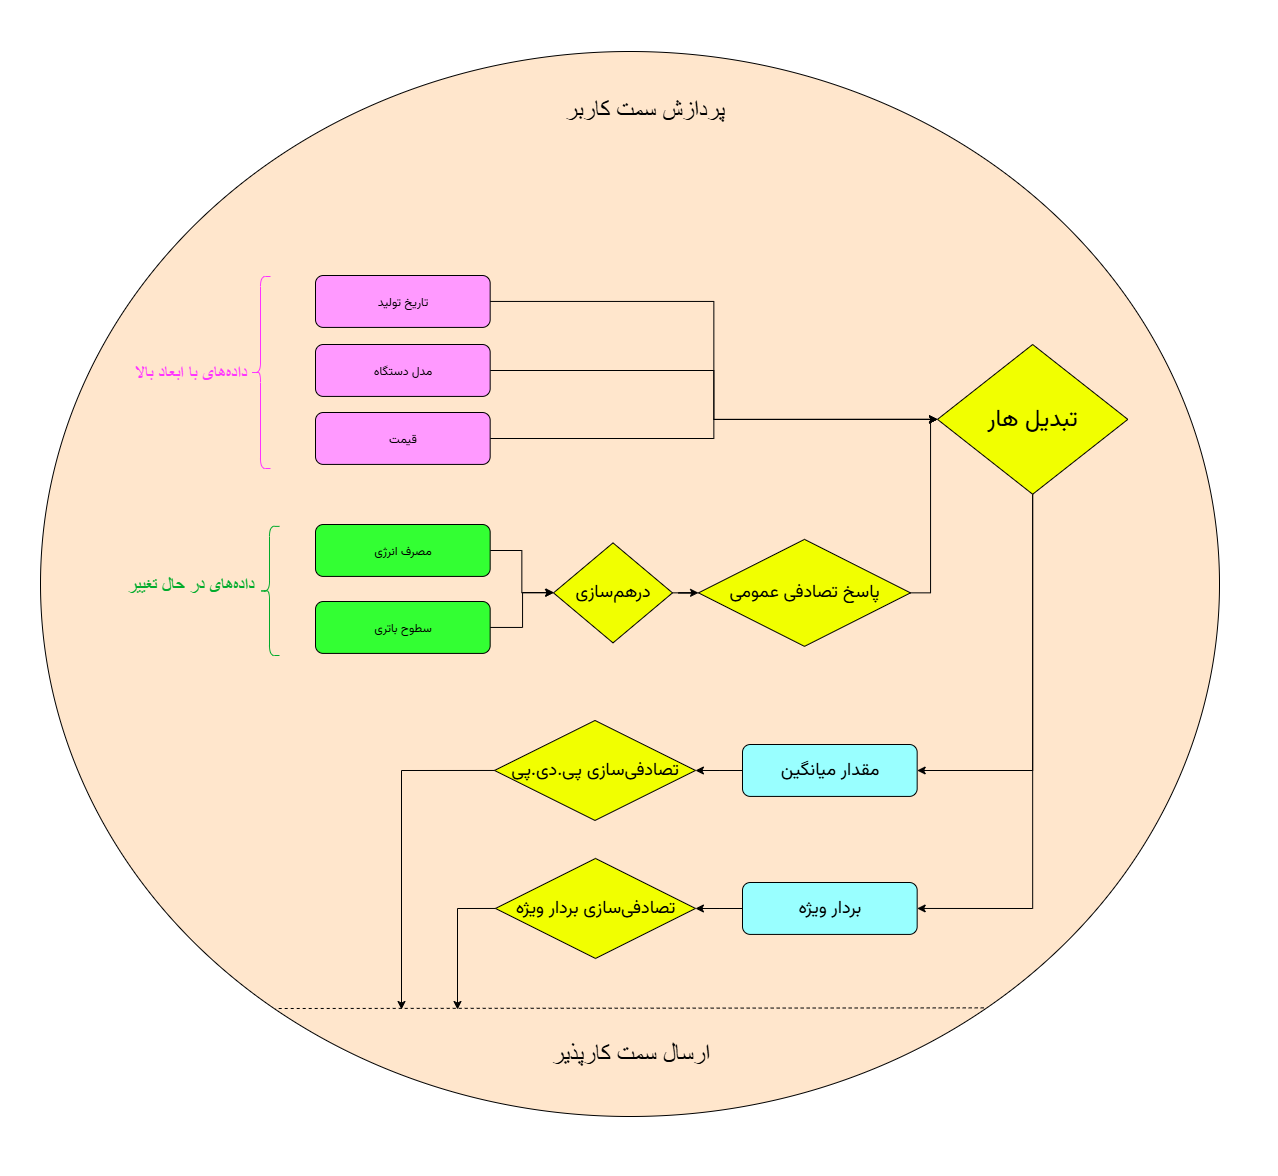
\includegraphics[width=0.9\textwidth]{figs/thesis-client.png}
  \caption{عملکرد روش پیشنهادی سمت کاربر}
  \label{fig:thesisClient}
\end{figure}


\زیرقسمت{فرایند مربوط به داده‌های در حال تغییر سمت کاربر}

پس از مشخص کردن داده‌های در حال تغییر، باید روش لولوها را روی این داده‌ها اعمال کنیم. هر کاربر یک تابع درهم‌ساز تصادفی انتخاب کرده و با استفاده از آن، دامنه‌ی داده‌ها را کاهش می‌دهد. درنتیجه چندین مقدار از دامنه اصلی به یک مقدار در دامنه کوچک نگاشت می‌شوند. این تصادم‌ها به صورت ذاتی یک لایه ابهام ایجاد می‌کنند که به حفظ حریم خصوصی کمک می‌کند. همچنین مطمئن می‌شویم که افزایش دامنه، تأثیر چندانی روی سودمندی نمی‌گذارد. سپس با کمک پاسخ تصادفی عمومی، شروع به آشفته‌سازی داده‌ها می‌کنیم. دقت کنید که این آشفته‌سازی از قوانین حفظ کردن پیروی می‌کند. الگوریتم \رجوع{الگوریتم: فرایند مربوط به یک بعد از داده‌های در حال تغییر سمت کاربر} این مرحله را به خوبی نمایش می‌دهد. 

در هنگام آشفته‌سازی مانند روش رپور از دو لایه تصافی‌سازی دائمی و آنی بهره گرفته و کاملا طبق الگوریتم \رجوع{الگوریتم: عملکرد لولوها سمت کاربر} پیاده‌سازی می‌شود. پس از این فرایند چند بعد از داده‌های ایمن ساخته‌ می‌شود و در کنار دیگر ابعاد ایستا به عنوان ورودی در فرایند اصلی قرار می‌گیرند.

\شروع{الگوریتم}{فرایند مربوط به یک بعد از داده‌های در حال تغییر سمت کاربر}
\ورودی مقادیر ورودی کاربر و متغیر در طول زمان $V = [v_1, v_2, \ldots, v_\tau]$ و بودجه‌های حریم خصوصی $\epsilon_\infty$ برای کل فرایند و $\epsilon_1$ برای تصادفی کردن یک گزارش واحد 
\خروجی بُعد نوفه‌دار شده با دامنه $g$

\دستور محاسبه‌ی اندازه دامنه‌ی جدید $g$ به صورت بهینه

\دستور انتخاب تابع درهم‌ساز $H$ به صورت تصادفی

\دستور کاهش دامنه: $hashed = H(V, g)$

\دستور تصادفی سازی: $perturbed = GRR(hashed, \epsilon_\infty, \epsilon_1)$

\دستور ارسال $perturbed$ سمت کارپذیر

\پایان{الگوریتم}

\زیرقسمت{فرایند اصلی مربوط به داده‌های با ابعاد بالا سمت کاربر}

ابتدا تمام داده‌ها باید در بازه‌‎ی $[-1, 1]$ یکنواخت\پانویس{Normalize} شوند. سپس با استفاده از تبدیل هار، داده‌های چند بعدی به دو مؤلفه مقدار میانگین و بردار ویژه تجزیه می‌شوند. مقدار میانگین با استفاده از روش پی.دی.پی نوفه‌دار می‌شود. به منظور تصادفی‌سازی بردار ویژه نیز از بهبودیافته‌ی الگوریتمی که در پی.پی.اِم.سی مطرح شد، استفاده ‌می‌کنیم. همچنین در هر دو تصادفی‌سازی از روش حفظ کردن بهره می‌گیریم تا هم در برابر پرسش‌های مکرر ایمن باشیم و هم سرعت عملیات را افزایش دهیم. در نهایت همگی داده‌ها برای کارپذیر ارسال می‌شوند. الگوریتم \رجوع{الگوریتم: فرایند اصلی مربوط به داده‌های با ابعاد بالا سمت کاربر} این مرحله را به صورت کلی نشان می‌دهد.

\شروع{الگوریتم}{فرایند اصلی مربوط به داده‌های با ابعاد بالا سمت کاربر}
\ورودی داده‌های با ابعاد بالا $A = [a_1, a_2, \ldots, a_d]$، دامنه تغییرات $domains$ و بودجه‌ی حریم خصوصی $\epsilon_\infty$
\خروجی میانگین و بردار ویژه به صورت نوفه‌دار شده

\دستور یکنواخت سازی در بازه‌ی $[-1, 1]$ : $normalized = normalize(A, domains)$

\دستور استخراج میانگین و بردار ویژه: $avg, eigenvector = HaarTransform(A)$

\دستور اضافه کردن نوفه به میانگین: $avg' = PDP(avg, \epsilon_\infty)$

\دستور اضافه کردن نوفه به بردار ویژه: $eigenvector' = improvedGPM(eigenvector, \epsilon_\infty)$

\دستور ارسال $avg'$ و $eigenvector'$ سمت کارپذیر

\پایان{الگوریتم}

\زیرقسمت{جمع‌آوری و تحلیل داده‌ها توسط کارپذیر}

کارپذیر پس از دریافت مقدار میانگین و بردار ویژه‌ی نوفه‌‌دار شده، معکوس تبدیل هار را اجرا کرده و داده‌هایی نزدیک به داده‌های اصلی را بدست می‌آورد. به منظور ارزیابی، روی داده‌های در حال تغییر تخمین شمارش صورت گرفته و روی دیگر ابعاد دو معیار احتمال توزیع داده‌ها و خطای مجذور میانگین\پانویس{Mean Square Error} اندازه‌گیری می‌شود.

از آنجایی که داده‌ها کاملا اعشاری هستند، باید ابتدا به نزدیک‌ترین مقدار صحیح رُند شده و سپس بر اساس روش تجمیع بیان‌شده در لولوها تخمین شمارش انجام شود. این اقدامات در الگوریتم فلان مشخص شده اند.


\شروع{الگوریتم}{جمع‌آوری و تحلیل داده‌ها توسط کارپذیر}
\ورودی میانگین $avg'$ و بردار ویژه $eigenvector'$ به صورت نوفه‌دار شده، تعداد ابعاد $d$ و دامنه تغییرات $domains$
\خروجی محاسبه‌ی تقریبی داده‌های اصلی به منظور انجام تحلیل آماری

\دستور بازگردانی ابعاد با کمک معکوس تبدیل هار: $\hat{D} = inverseHaar(avg', eigenvector', d)$

\دستور بازگردانی داده‌ها به بازه‌ی اصلی: $\hat{D} = denormalize(\hat{D}, domains)$

\دستور استفاده از $\hat{D}$ به منظور انجام تحلیل‌های آماری

\دستور جداسازی ابعاد در حال تغییر: $\hat{E} = \hat{D}\{d_i | d_i \hspace{5pt} \text{evolving is}\}$

\دستور رُند کردن به نزدیک‌ترین مقدار صحیح: $rounded = round(\hat{E})$

\دستور تخمین شمارش روی $\hat{E}$ با استفاده از فرمول \رجوع{equ:estimateFrequency}

\پایان{الگوریتم}

\قسمت{محاسبه‌ی اندازه دامنه‌ی جدید به صورت بهینه}

مقدار $g$ در پروتکل لولوها، اندازه دامنه جدید و کاهش‌یافته است که از طریق درهم‌سازی به دست می‌آید. انتخاب درست $g$ تعادل بین حریم خصوصی و سودمندی را برقرار می‌کند. با کاهش این مقدار ذکر شده، حریم خصوصی افزایش میابد ولی سودمندی افت خواهد کرد. از طرفی بزرگ بودن دامنه، باعث کاهش تصادم‌ها شده و در نتیجه، سودمندی افزایش میابد.

در آمار، سودمندی یا دقت یک تخمین‌گر، معمولاً به صورت معکوس با واریانس آن سنجیده می‌شود. واریانس بالا یعنی تخمین‌های ما پراکندگی زیادی حول مقدار واقعی دارند و غیرقابل اعتماد هستند. از طرفی واریانس پایین به این معناست که تخمین‌های ما به مقدار واقعی بسیار نزدیک هستند. بنابراین، هدف ما انتخاب یک $g$ مناسب است که به موجب آن، واریانس تخمین شمارش کمینه شود.


با توجه به فرمول \رجوع{equ:estimateFrequency} که تخمین شمارش بر اساس ورودی‌های پاسخ تصادفی عمومی را بیان می‌کند، می‌توان مقدار واریانس را به صورت تقریبی بدست آورد:

\begin{equation}
\mathbb{V}^*[\hat{f}_L(v)] = \frac{(p_2q_1 - q_2(q_1-1))(-p_2q_1 + q_2(q_1-1)+1)}{n(p_1-q_1)^2(p_2-q_2)^2}
\end{equation}

برای پیدا کردن نقطه‌ای که یک تابع در آن کمینه می‌شود، از مشتق استفاده می‌کنیم. پس از تابع واریانس نسبت به $g$ مشتق گرفته و برابر صفر قرار می‌دهیم تا نقاط بحرانی را پیدا کنیم.

$$\frac{\partial V^*(g)}{\partial g} = 0$$

با حل معادله‌ی بالا، مقدار بهینه‌ی $g$ را بدست می‌آوریم. برای ساده‌تر کردن نمایش فرمول نهایی، از دو متغیر کمکی استفاده شده است.

$$b = e^{\epsilon_\infty}, \quad a = e^{\epsilon_1}$$
\begin{equation}
g_{\text{optimal}} = 1 + \max\left(1, \left\lfloor \frac{1-a^2+\sqrt{a^4-14a^2+12ab(1-ab)+12a^3b+1}}{6(a-b)} \right\rfloor \right)
\end{equation}
\قسمت{درهم‌سازی}

برای پیاده‌سازی الگوریتم درهم‌سازی از کتابخانه‌ی ایکس.ایسک.هش\پانویس{xxhash} \مرجع{XxhashCitekeyMisc} در پایتون\پانویس{python} استفاده می‌کنیم. این کتابخانه از الگوریتمی استفاده می‌کند که سرعت بالایی داشته و عملکرد بهتری نسبت به الگوریتم‌هایی مانند اِم.دی.5\پانویس{MD5} و شا.وان\پانویس{SHA-1} دارد. این الگوریتم در مواردی مانند بررسی یکپارچگی داده‌ها، شناسایی فایل‌های تکراری و عملیات جستجو که سرعت در آنها اهمیت بالایی دارد، بسیار مناسب است.

قطعه کد \رجوع{code:xxhash} با استفاده از الگوریتم ایکس.ایسک.اچ.32\پانویس{xxh32}، هر یک از مقادیر موجود در ردیف داده‌های کاربر را به یک عدد صحیح درهم‌سازی کرده و سپس با استفاده از عملیات باقیمانده، آن را به یک محدوده مشخص نگاشت می‌دهد. این تابع یک مقدار اولیه $seed$ به عنوان ورودی درهم‌ساز دریافت می‌کند. مقدار اولیه برای هر کاربر به صورت تصادفی تولید می‌شود. در نتیجه ما از این عدد به عنوان تابع درهم‌ساز شخصی کاربران یاد می‌کنیم.

\LRE{
\begin{lstlisting}[language=Python, label=code:xxhash]
def reduce_domain_row(user_data_row, g, user_hash_function):
    return [
      (xxhash.xxh32(str(value), seed=user_hash_function).intdigest() % g)
      for value in user_data_row
    ]
\end{lstlisting}
}

\قسمت{یکنواخت‌سازی}

روش پی.پی.اِم.سی از تمام ابعاد میانگین گرفته و سمت کارپذیر می‌فرستد. در میانگین‌گیری اگر مقدار یک بُعد با اختلاف زیادی بیشتر از دیگر ابعاد باشد، نتیجه به سمت آن ویژگی سو می‌گیرد. پس قبل از تبدیل هار تمام ابعاد باید در یک بازه‌ی مشخص قرار گیرند. در روش پیشنهادی مانند الگوریتم پی.پی.اِم.سی تمام ابعاد در بازه‌ی $[-1, 1]$ یکنواخت می‌شوند.

این عملیات طبق کد \رجوع{code:normalization} با استفاده از روش مقیاس‌بندی کمینه-بیشینه\پانویس{Min-Max Normalization} پیاده‌سازی شده است.

\LRE{
\begin{lstlisting}[language=Python, label=code:normalization]
def normalize(x, domain):
    max_domain = max(domain)
    min_domain = min(domain)
    return ((2*(x-min_domain)) / (max_domain-min_domain)) - 1
\end{lstlisting}
}

\قسمت{بهبود روش جی.پی.اِم}

الگوریتم \رجوع{الگوریتم: سازوکار آشفته‌سازی بردار ویژه} روش جی.پی.اِم را به طور کامل توضیح داده است. خط 3 این الگوریتم تمام مقادیری از بردار ویژه که کمتر از حد آستاته هستند را صفر کرده و نوفه‌ای روی آنها اعمال نمی‌کند. از آنجایی که نوفه‌ی اضافی حذف شده است، سودمندی کمی بهبود یافته است ولی با صفر کردن این مقادیر، دقت نهایی به دشت افت خواهد کرد. فرض کنید تعداد زیادی از عناصر بردار ویژه مقداری کمتر از حد آستانه دارند؛ در این صورت تمام این عناصر مقدار صفر پیدا کرده و با انجام معکوس تبدیل هار، نتیجه اختلاف زیادی با مقدار اصلی پیدا می‌کند.

شاید با پیدا کردن حد آستانه مناسب بتوانیم مشکل ذکر شده را حل کنیم؛ ولی حد آستانه‌ی مناسب کاملا وابسته به داده‌ها و نوع اطلاعاتی است که کاربران ذخیره می‌کنند. اگر بخواهیم الگوریتم مستحکمی ارائه دهیم که با کمترین تغییر اکثر نیازمندی‌های ما را پوشش دهد، باید روش دیگری اتخاذ کنیم.

به منظور پیدا کردن راهکاری مناسب برای رسیدن به دقت بالاتر، کافیست این مقادیر کمتر از حد آستانه در همان مقدار خود باقی بمانند و فقط نوفه روی آنها اعمال نشود. نتایج ارزیابی روی چند مجموعه داده‌ی مختلف نشان داده است که این راهکار با حفظ حریم خصوصی تفاضلی، سودمندی بهتری خواهد داشت.

$$\tilde{e}_i = 
\begin{cases} 
e_i, & |e_i| \leq \theta \\
\text{from random at uniformly Sample} \hspace{5pt} [\frac{e_i \cdot e^{\epsilon}-1}{e^{\epsilon}-1}, \frac{e_i \cdot e^{\epsilon}+1}{e^{\epsilon}-1}], & v_i = 0 \\
\text{from random at uniformly Sample} \hspace{5pt} [-\frac{e^{\epsilon}+1}{e^{\epsilon}-1}, \frac{e_i \cdot e^{\epsilon}-1}{e^{\epsilon}-1}) \cup (\frac{e_i \cdot e^{\epsilon}+1}{e^{\epsilon}-1}, \frac{e^{\epsilon}+1}{e^{\epsilon}-1}], & v_i = 1 
\end{cases}$$


\قسمت{تضمین حریم خصوصی تفاضلی}

در این بخش به اثبات ریاضی امن بودن روش پیشنهادی می‌پردازیم. روش پیشنهادی از دو راهکار تبدیل هار و درهم‌سازی محلی استفاده شده است. در راهکار تبدیل هار، از دو سازوکار آشفته‌سازی پی.دی.پی و جی.پی.اِم استفاده می‌شود. در ادامه اثبات امن بودن این دو سازوکار بیان می‌شود.

\زیرقسمت{اثبات امن بودن سازوکار جی.پی.اِم}

سازوکار آشفته‌سازی سراسری برای حفاظت از حریم خصوصی بردار ویژه طراحی شده است. در این سازوکار، مجموعه‌ای شامل بردارهای دودویی به صورت تصادفی و مستقل از ورودی ساخته می‌شود. سپس به دو مجموعه‌ی $A$ و $B$ افراز خواهد شد. مجموعه‌ی $A$ شامل تمام بردارهایی است که تعداد اعضای 1 در آن‌ها زوج است. همچنین مجموعه‌ی $B$ شامل تمام بردارهایی است که تعداد اعضای 1 در آن‌ها فرد است. بر اساس قضیه‌ی دوجمله‌ای اندازه‌ی این دو مجموعه کاملا برابر خواهد بود. سپس یک متغیر تصادفی $X$ تعریف می‌شود که با احتمالی وابسته به $\epsilon$، یکی از دو مجموعه $A$ یا $B$ را انتخاب کرده و یک بردار به صورت تصادفی از مجموعه‌ی انتخاب شده استخراج می‌شود. در نهایت بر اساس بردار استخراج شده، بردار ویژه نوفه‌دار می‌شود.
 
برای اثبات باید نسبت احتمال تولید خروجی یکسان برای ورودی‌های متفاوت را بدست آوریم و نشان دهیم که این عدد کوچکتر یا مساوری $e ^ \epsilon$ خواهد بود. اکنون می‌خواهیم نسبت احتمال را برای یک خروجی دلخواه $y$ بررسی کنیم.

$$\Pr[X = 1] = \frac{e^{\varepsilon}}{e^{\varepsilon} + 1}
\quad
\Pr[X = 0] = \frac{1}{e^{\varepsilon} + 1}$$
$$
\Pr[y = v \mid V] =
\begin{cases}
\dfrac{e^{\varepsilon}}{e^{\varepsilon}+1} \cdot \dfrac{1}{|A|}, & v \in A, \\[10pt]
\dfrac{1}{e^{\varepsilon}+1} \cdot \dfrac{1}{|B|}, & v \in B .
\end{cases}$$

نسبت خروجی در بدترین حالت برای دو ورودی از دو مجموعه‌ی مختلف به صورت زیر بدست‌ می‌آید.
$$
\text{since } \hspace{5pt} |A| = |B|, \quad
\frac{\dfrac{e^{\varepsilon}}{e^{\varepsilon}+1}\cdot \dfrac{1}{|A|}}
     {\dfrac{1}{e^{\varepsilon}+1}\cdot \dfrac{1}{|B|}}
\;\;=\;\;
\frac{\dfrac{e^{\varepsilon}}{e^{\varepsilon}+1}}
     {\dfrac{1}{e^{\varepsilon}+1}}
\;\;=\;\; e^{\varepsilon}
$$

عبارت بالا نشان می‌دهد که مقدار بدست آمده همیشه کمتر از $e ^ \epsilon$ است. بنابراین سازوکار جی.پی.اِم به دلیل ساختار احتمالی و مستقل از ورودی خود، حریم خصوصی را تضمین می‌کند.

\زیرقسمت{اثبات امن بودن سازوکار پی.دی.پی}

سازوکار تصادفی یک مقدار آشفته‌شده را از یک توزیع احتمالی تولید می‌کند که شکل آن به ورودی الگوریتم بستگی دارد. توزیع احتمال به این صورت است که در ناحیه‌ی نزدیک به مقدار ورودی، احتمال انتخاب خروجی بیشتر از نواحی دیگر خواهد بود. برای اثبات $\epsilon{-}LDP$ بودن الگوریتم، باید نسبت تولید یک خروجی یکسان برای دو ورودی دلخواه را محاسبه کرده و بیشترین مقدار ممکن این نسبت را پیدا کنیم. بیشترین مقدار زمانی حاصل می‌شود که خروجی داخل بازه‌ی نزدیک به ورودی اول بوده و همچنین خارج از بازه‌ی نزدیک به ورودی دوم باشد: 


$$\frac{Pr[M(m_1) = y]}{Pr[M(m_2) = y]} = \frac{q.e^\epsilon}{q} = e^\epsilon$$


\زیرقسمت{اثبات امن بودن درهم‌سازی محلی}

در روش درهم‌سازی محلی از سازوکار تصادفی‌سازی عمومی برای نوفه‌دار کردن داده استفاده می‌شود. این سازوکار با توجه به مقادیر انتخابی $p$ و $q$، حریم خصوصی تفاضلی محلی را ارضا می‌کند. نحوه‌ی تنظیم این مقادیر در توضیح روش لولوها \رجوع{equ:set-p-q} به تفصیل بیان شده است.

\زیرقسمت{نتیجه‌گیری}

نشان دادیم که سازوکارهای مذکور همگی حریم خصوصی تفاضلی محلی را ارضا می‌کنند. روی داده‌های غیر پویا تنها سازوکارهای جی.پی.اِم و پی.دی.پی اجرا می‌شوند. پس با توجه به امن بودن چنین سازوکارهایی، می‌توان گفت حریم خصوصی برای داده‌های غیر پویا تضمین می‌شود. از طرفی روی داده‌های در حال تغییر هر سه سازوکار جی.پی.اِم، پی.دی.پی و تصادفی‌سازی عمومی به صورت متوالی انجام می‌شوند. این عملیات شامل قانون ترکیب متوالی نخواهد شد؛ زیرا ورودی سازوکارهای جی.پی.اِم و پی.دی.پی، خروجی سازوکار تصادفی‌سازی عمومی هستند و نمی‌‌توان گفت هر سه سازوکار روی یک داده‌ی ورودی اجرا می‌شوند. بنابراین می‌توان نتیجه گرفت راهکار پیشنهادی با موفقیت حریم خصوصی تفاضلی محلی را ارضا می‌کند.







